\section{Introduction}
\label{s:intro}

%\wajih{I have updated the macro logs as it does not make sense to use \ logs for just "system". I have changed the macro to "system logs". Make sure the paper is consistent with that.}

% The effectiveness of IDSes hinges on their ability to accurately detect these threats, maintain low false positive rates, and operate with minimal resource consumption, ensuring system performance is not compromised.

%\wajih{Give the workflow of MSSP and cite that organizations outsource their security. If you find any numbers on how many comapnies use MSSP and outsource their security operations that would be great. If you find any realworld attack examples on MSSP where the data was leaked that would be great as well. }

Intrusion Detection Systems (IDSes) play an essential role in enterprise security strategies to counteract Advanced Persistent Threats (APTs). APTs are notably stealthy and persistent, exemplified by the significant system disruptions seen in attacks such as Solar Winds~\cite{solarwinds} and NotPetya~\cite{notpetya}. To defend against these attacks, many organizations outsource their security operations to different MSSPs. A study~\cite{msspsurvey}  of more than 5,000 IT professionals found that nearly three in every four companies are turning to MSSPs The MSSP integrates their security tools with the client's systems to collect \logs. This involves configuring the client’s systems to send \logs to the cloud for threat detection. Figure~\ref{mssp} shows the architecture for MSSP operations.

Data Provenance techniques have been increasingly used in IDSes to detect system intrusions. By analyzing system logs and converting them into provenance graphs, these systems offer a comprehensive view of system execution. Provenance-based IDSes~\cite{streamspot,provdetector2020,wang2022threatrace,shadewatcher,yangprographer,han2020unicorn} have emerged as a potent solution, utilizing the rich context within \logs to improve detection capabilities. The MSSP can leverage these recent advancements for automated threat detection without requiring attack signatures.

%\wajih{Please put the MSSP figure we talk about here.}

\begin{figure}[t!]
    \centering
    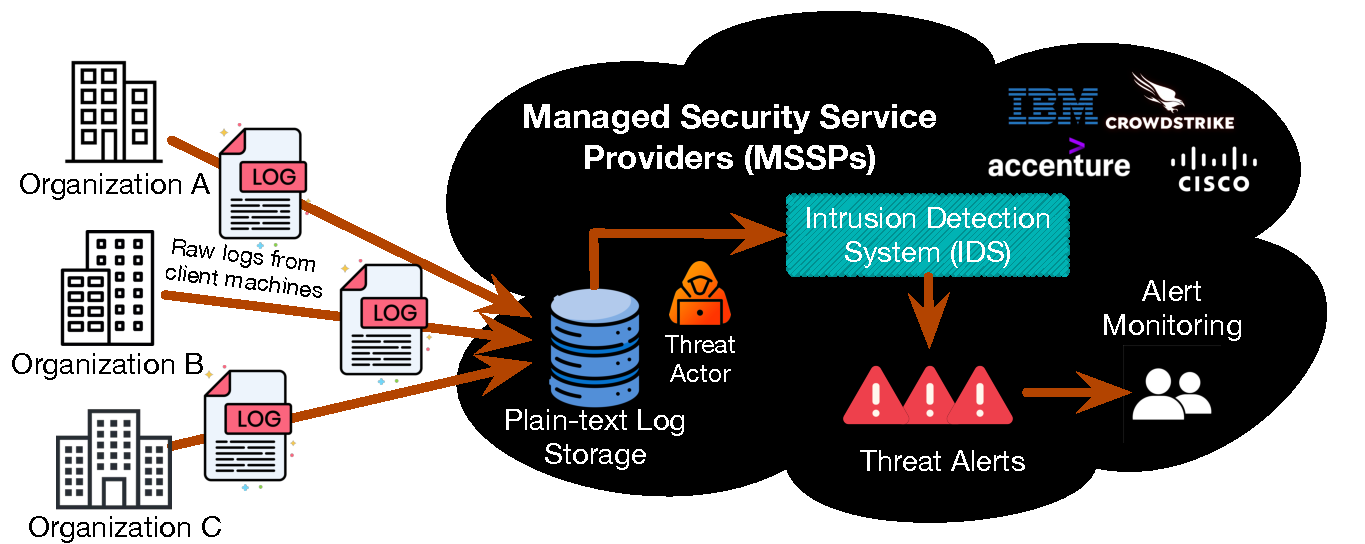
\includegraphics[width=0.4\textwidth]{fig/mssp.pdf}
    \caption{The MSSP architecture for intrusion detection. The logs are collected from clients and then analyzed for any threats.}
    \label{mssp}
    \vspace{-2ex}
  \end{figure}  

Despite their promise, the current mode of operation of MSSP and the above-mentioned techniques for detecting intrusions face significant challenges in the complex landscape of enterprise security:

\smallskip
\noindent
\textbf{C1: Lack of Privacy Preservation:} The current mode of operation of MSSPs and traditional provenance-based IDSes (PIDS)~\cite{flash2024,cheng2023kairos,wang2022threatrace} rely on a centralized infrastructure, necessitating client machines to transmit their log data to a central server. \flash~\cite{flash2024} and \kairos~\cite{cheng2023kairos} are some recent state-of-the-art PIDS that operate in a centralized manner, assuming the \logs from different machines will be present in a centralized location where these systems are operational. This approach risks user privacy as \logs encompass detailed records of system execution, including sensitive information and activity patterns. This information can include specific urls visited, ip addresses and the applications user is using. These privacy concerns have been underscored in a report by Datadog~\cite{datadog}, a prominent provider of system monitoring services.
    
\smallskip
\noindent
\textbf{C2: Excessive Network Overhead:} In MSSP setting, \logs need to be send over network for threat detection. The logs from modern systems can accumulate to gigabytes per day, resulting in significant network costs for both users and organizations. Our analysis of \flash and \kairos, utilizing the \optc dataset as detailed in Section~\ref{cost_metric}, illustrates this point. For an organization similar to the one represented in the \optc dataset, with a comparable number of hosts, the total volume of logs transmitted daily would reach 1000 GB. This volume of data could lead to substantial network expenses daily. Moreover, it poses a challenge for users with limited network bandwidth to upload this volume of data efficiently.
    
    % \item[--] \textbf{C2: Excessive Network Overhead:} In MSSP setting, \logs logs need to be send over network for threat detection. The logs from modern systems can accumulate to gigabytes per day, resulting in significant network costs for both users and organizations. Additionally, the need for extensive disk storage to house these logs adds complexity. Current PIDS models fail to address these challenges, undermining their practical applicability. Our analysis of \flash and \kairos, utilizing the \optc dataset as detailed in Section~\ref{cost_metric}, illustrates this point. For an organization similar to the one represented in the \optc dataset, with a comparable number of hosts, the total volume of logs transmitted daily would reach 1000 GB. This volume of data could lead to substantial network and storage expenses daily. Moreover, it poses a significant challenge for users with limited network bandwidth to upload this volume of data efficiently.
    %\wajih{Could you give specific numbers about network overhead and disk overhead that would be great.} \wajih{Again cite existing PIDS with names that would suffer from this issue.}

\smallskip
\noindent
\textbf{C3: Scalability Challenges:} The centralized approach employed by current PIDS poses scalability challenges as the number of hosts within an organization grows. Such centralization serves as a bottleneck, leading to log congestion and thereby impeding efficient intrusion detection at scale. Additionally, for large organizations, the centralized accumulation of logs can lead to significant disk storage overhead. To accommodate an increasing number of hosts, organizations must continually allocate more resources. Consequently, the existing approach to threat detection lacks inherent scalability. Our evaluations of \flash and \kairos demonstrate that these systems would face log congestion in organizations of a size comparable to that represented by the \optc dataset. As detailed in Section~\ref{sec:eval}, \flash would require 27.7 hours, and \kairos 56.6 hours, to process a single day's worth of logs from the \optc dataset.
    
    %\wajih{Again you need to add more details here about scalability issues. Having specific numbers for existing PIDS is important. Also cite those existing PIDS }


%\wajih{I added C1, C2, C3 with each challenge above. You need to refer to each of the challenge below and tell how you solve that challenge. Something like: "To address C1, we do blah blah"}

To address these challenges, we introduce \Sys, that combines provenance graph representation learning with federated learning (FL). In \Sys, client logs remain local, preserving user privacy (C1). Each client independently trains \gnnshort models, which are subsequently aggregated with models from other clients on a central server, capturing activity patterns across organizations.

In \Sys, network overhead is minimal, as logs are not transmitted to the cloud. The only network costs arise from transmitting model updates to the server. These updates, merely a few kilobytes per client, do not significantly burden the client or the organization's network (C2). The primary computation for \Sys, both during training and inference, occurs locally on client machines. Clients utilize their local compute resources to train models on provenance graphs constructed from their logs. For threat detection post-training, clients run \Sys locally to generate alerts. This design allows our system to scale naturally with the addition of more hosts, as each client leverages its own computing power and disk storage, addressing challenge (C3).

% To tackle these challenges, we introduce \Sys, a novel PIDS that merges provenance graph representation learning with FL. This hybrid approach facilitates efficient and precise detection of Advanced Persistent Threat (APT) attacks in a decentralized fashion. The client local logs data do not need to be transmitted over the network and stored at a centralized storage (C2). In \Sys, each client uses its local compute power to run the \Sys anomaly detection module. Thus, our system is naturally scalable (C3) with the number of host machines added to the network.

%\wajih{I will describe FL and associated challenges after introducing your methodology because it is your idea. Just like we discussed in our last lab meeting.}

%\wajih{The transition of this paragraph is not great. You already talked about solving changes above and then you again talk about solving challenges below. }

The application of FL to develop a privacy-preserving PIDS presents several challenges. In a federated setting, separate models are trained on each client and then aggregated to form a unified model. These clients often have divergent data distributions due to running different application sets. Merging these models with heterogeneous distributions into a single global model through a mean aggregation operation leads to the conflation of distinct patterns, resulting in suboptimal performance. Additionally, variations in the amount of \logs across clients cause data imbalances within the organization. In such cases, contributions from clients with less data are often overshadowed by those with more data.

To address heterogeneity and data imbalance, we develop a \gnnshort ensemble learning framework. Here, system processes across all clients are standardized into \textit{K} bins in a privacy preserving fashion. Each client then organizes its process nodes according to these bins, constructs a provenance subgraph for each bin, and trains a \gnnshort model. Subsequently, the \textit{K} model pairs from all clients are aggregated to form a global ensemble model set. This approach ensures that models with similar distributions are merged, preserving unique activity patterns, and enhances the likelihood of conserving patterns from clients with less data.

Recent works such as \flash have demonstrated the effectiveness of using semantic attributes from \logs to generate context-rich feature vectors for model training. In a federated setting, when each client trains their own semantic encoder, such as \wordvec, to produce semantic input features, the global \gnnshort models tend to underperform. This issue arises because different models encode varying information for the same tokens, necessitating aggregation to achieve unified vector representations. However, encoders like \wordvec may contain sensitive data, including process names, IP addresses, and file names. To maintain privacy, these models cannot be sent to a central server. To solve this challenge, we employ a two-server architecture where the central server issues encryption keys for the clients to encode \wordvec tokens, and a utility server processes the encrypted tokens to merge them in a privacy preserving manner.

%\wajih{Add one paragraph how you solve that above mentioned challenge. This will highlight the novelty of your system.}

%\wajih{make sure to say two or three lines about adversarial attacks and say that more details are present in the discussion section.}

%\wajih{Add one paragraph related to evaluation results.}

We have conducted extensive evaluations of our system's effectiveness using open-source datasets from \darpa, specifically E3~\cite{darpae3}, E5~\cite{darpae5}, and \optc~\cite{anjum2021analyzing}. These datasets encompass a broad spectrum of attack scenarios and system behaviors. Our findings indicate that \Sys achieves high detection performance, with an average precision of 96\% and recall of 97\%. Thus, our system performs comparably to state-of-the-art centralized systems like \flash and \kairos. As detailed in section~\ref{cost_metric}, our system achieves a 170-fold reduction in communication and storage costs compared to \flash and \kairos. Since our technique is decentralized, our inference time is bounded by the client with the most log data; it will only take approximately 3 minutes to run inference on the complete \optc dataset, whereas \flash and \kairos take many hours. Employing FL exposes our system to certain types of adversarial attacks, such as model poisoning, inference, and gradient attacks. We provide a comprehensive analysis of our system's resilience against these attacks in section~\ref{sec:discussion}. We also present a detailed analysis of the privacy protection of our system in section~\ref{privacy}.

%\wajih{Add list of main contributions}
The main contributions of our work are as follows:

\begin{itemize}[topsep=.1ex,itemsep=-.1ex,leftmargin=*]
    \item We are the first to introduce a Federated Graph Learning-based PIDS, \Sys, which is privacy-preserving, highly scalable, and offers impressive detection performance.
    \item We have introduced a novel multi-server architecture and an encryption scheme to prevent the central server from leaking user privacy.
    \item We offer a novel \gnnshort ensemble framework personalized at the system entity level to deal with heterogeneous and imbalanced clients.
    \item We conduct a comprehensive evaluation of our technique on real-world datasets. The results highlight \Sys's effectiveness in identifying malicious activities and its high scalability compared to existing systems.
\end{itemize}

\PP{Open Source Commitment} To advance threat detection research and ensure reproducibility, we plan to release the source code of \Sys publicly upon the publication of this paper.